

\tikzset{every picture/.style={line width=0.75pt}} %set default line width to 0.75pt        

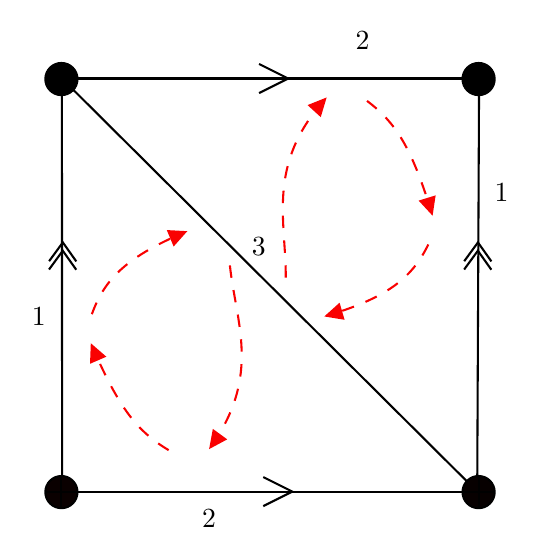
\begin{tikzpicture}[x=0.75pt,y=0.75pt,yscale=-1,xscale=1]
%uncomment if require: \path (0,487); %set diagram left start at 0, and has height of 487

%Straight Lines [id:da8215288959193072] 
\draw    (100,121) -- (100.08,320) ;
%Straight Lines [id:da8526418629967348] 
\draw    (301,120) -- (300.08,320) ;
%Straight Lines [id:da5367620041050422] 
\draw    (100.08,320) -- (300.08,320) ;
%Straight Lines [id:da4784595305292364] 
\draw    (100,121) -- (300,121) ;
\draw   (93.79,213.01) -- (100.41,203.96) -- (106.89,213.11)(93.82,209.01) -- (100.44,199.96) -- (106.92,209.11) ;
\draw   (293.79,213.01) -- (300.41,203.96) -- (306.89,213.11)(293.82,209.01) -- (300.44,199.96) -- (306.92,209.11) ;
\draw   (195,114) -- (209,121) -- (195,128) ;
\draw   (197,313) -- (211,320) -- (197,327) ;
%Straight Lines [id:da22151170816098675] 
\draw    (100,121) -- (300.08,320) ;
\draw  [fill={rgb, 255:red, 0; green, 0; blue, 0 }  ,fill opacity=1 ] (92,121.25) .. controls (92,116.97) and (95.47,113.5) .. (99.75,113.5) .. controls (104.03,113.5) and (107.5,116.97) .. (107.5,121.25) .. controls (107.5,125.53) and (104.03,129) .. (99.75,129) .. controls (95.47,129) and (92,125.53) .. (92,121.25) -- cycle ; \draw   (92,121.25) -- (107.5,121.25) ; \draw   (99.75,113.5) -- (99.75,129) ;
\draw  [fill={rgb, 255:red, 0; green, 0; blue, 0 }  ,fill opacity=1 ] (293,121.25) .. controls (293,116.97) and (296.47,113.5) .. (300.75,113.5) .. controls (305.03,113.5) and (308.5,116.97) .. (308.5,121.25) .. controls (308.5,125.53) and (305.03,129) .. (300.75,129) .. controls (296.47,129) and (293,125.53) .. (293,121.25) -- cycle ; \draw   (293,121.25) -- (308.5,121.25) ; \draw   (300.75,113.5) -- (300.75,129) ;
\draw  [fill={rgb, 255:red, 10; green, 0; blue, 0 }  ,fill opacity=1 ] (92,320.25) .. controls (92,315.97) and (95.47,312.5) .. (99.75,312.5) .. controls (104.03,312.5) and (107.5,315.97) .. (107.5,320.25) .. controls (107.5,324.53) and (104.03,328) .. (99.75,328) .. controls (95.47,328) and (92,324.53) .. (92,320.25) -- cycle ; \draw   (92,320.25) -- (107.5,320.25) ; \draw   (99.75,312.5) -- (99.75,328) ;
\draw  [fill={rgb, 255:red, 7; green, 0; blue, 0 }  ,fill opacity=1 ] (293,320.25) .. controls (293,315.97) and (296.47,312.5) .. (300.75,312.5) .. controls (305.03,312.5) and (308.5,315.97) .. (308.5,320.25) .. controls (308.5,324.53) and (305.03,328) .. (300.75,328) .. controls (296.47,328) and (293,324.53) .. (293,320.25) -- cycle ; \draw   (293,320.25) -- (308.5,320.25) ; \draw   (300.75,312.5) -- (300.75,328) ;
%Curve Lines [id:da13696914158614193] 
\draw [color={rgb, 255:red, 249; green, 1; blue, 1 }  ,draw opacity=1 ] [dash pattern={on 4.5pt off 4.5pt}]  (114.42,234.54) .. controls (120.24,218.54) and (129.82,207.71) .. (157.77,195.66) ;
\draw [shift={(160.42,194.54)}, rotate = 157.38] [fill={rgb, 255:red, 249; green, 1; blue, 1 }  ,fill opacity=1 ][line width=0.08]  [draw opacity=0] (8.93,-4.29) -- (0,0) -- (8.93,4.29) -- cycle    ;
%Curve Lines [id:da42631957373483753] 
\draw [color={rgb, 255:red, 249; green, 1; blue, 1 }  ,draw opacity=1 ] [dash pattern={on 4.5pt off 4.5pt}]  (151.42,300.04) .. controls (135.9,290.83) and (127.43,279.26) .. (115.07,251.19) ;
\draw [shift={(113.92,248.54)}, rotate = 66.57] [fill={rgb, 255:red, 249; green, 1; blue, 1 }  ,fill opacity=1 ][line width=0.08]  [draw opacity=0] (8.93,-4.29) -- (0,0) -- (8.93,4.29) -- cycle    ;
%Curve Lines [id:da5983276540829184] 
\draw [color={rgb, 255:red, 249; green, 1; blue, 1 }  ,draw opacity=1 ] [dash pattern={on 4.5pt off 4.5pt}]  (180.92,211.04) .. controls (183.86,238.48) and (195.92,263.52) .. (172.4,297.45) ;
\draw [shift={(170.92,299.54)}, rotate = 306.08] [fill={rgb, 255:red, 249; green, 1; blue, 1 }  ,fill opacity=1 ][line width=0.08]  [draw opacity=0] (8.93,-4.29) -- (0,0) -- (8.93,4.29) -- cycle    ;
%Curve Lines [id:da9247996561877188] 
\draw [color={rgb, 255:red, 249; green, 1; blue, 1 }  ,draw opacity=1 ] [dash pattern={on 4.5pt off 4.5pt}]  (276.54,200.95) .. controls (268.99,216.21) and (258.27,225.92) .. (229.16,234.81) ;
\draw [shift={(226.41,235.63)}, rotate = 343.71] [fill={rgb, 255:red, 249; green, 1; blue, 1 }  ,fill opacity=1 ][line width=0.08]  [draw opacity=0] (8.93,-4.29) -- (0,0) -- (8.93,4.29) -- cycle    ;
%Curve Lines [id:da42565795945334595] 
\draw [color={rgb, 255:red, 249; green, 1; blue, 1 }  ,draw opacity=1 ] [dash pattern={on 4.5pt off 4.5pt}]  (246.99,131.77) .. controls (261.4,142.64) and (268.53,155.07) .. (277.72,184.32) ;
\draw [shift={(278.58,187.09)}, rotate = 252.9] [fill={rgb, 255:red, 249; green, 1; blue, 1 }  ,fill opacity=1 ][line width=0.08]  [draw opacity=0] (8.93,-4.29) -- (0,0) -- (8.93,4.29) -- cycle    ;
%Curve Lines [id:da31674209595039604] 
\draw [color={rgb, 255:red, 249; green, 1; blue, 1 }  ,draw opacity=1 ] [dash pattern={on 4.5pt off 4.5pt}]  (207.85,216.97) .. controls (207.96,189.37) and (198.73,163.16) .. (225.84,132.02) ;
\draw [shift={(227.55,130.11)}, rotate = 132.41] [fill={rgb, 255:red, 249; green, 1; blue, 1 }  ,fill opacity=1 ][line width=0.08]  [draw opacity=0] (8.93,-4.29) -- (0,0) -- (8.93,4.29) -- cycle    ;

% Text Node
\draw (84,230) node [anchor=north west][inner sep=0.75pt]   [align=left] {1};
% Text Node
\draw (307,170) node [anchor=north west][inner sep=0.75pt]   [align=left] {1};
% Text Node
\draw (166,327) node [anchor=north west][inner sep=0.75pt]   [align=left] {2};
% Text Node
\draw (240,97) node [anchor=north west][inner sep=0.75pt]   [align=left] {2};
% Text Node
\draw (190,196) node [anchor=north west][inner sep=0.75pt]   [align=left] {3};


\end{tikzpicture}
